\documentclass[11pt,a4paper]{article}
\usepackage{geometry,url,graphicx,float,amsmath,xcolor,listings}
\newcommand{\highlight}[1]{\colorbox{gray}{$\displaystyle#1$}}
\newcommand{\head}[1]{\textnormal{\textbf{#1}}}

\begin{document}
	\title{Support Vector Machines for Face Recognition \\ using \texttt{scikit-learn}}
	\author{CS 280 Mini Project\\Joshua Frankie B. Rayo\\2011-19612}
	\maketitle
	\tableofcontents
	\listoffigures
	\lstlistoflistings
	
	\section{Introduction}
	Image classification, particularly face recognition is one of the important applications of using intelligent systems. Facial images of different people are used to train a model hoping to recognize familiar faces in the future. Supervised learning is possible using artificial neural networks (ANN) and support vector machines (SVM), while unsupervised learning is possible using eigenfaces from principal component analysis.
	
	ANN implements the empirical risk minimization pprinciple that seeks to minimize the misclassification error of the training data, while SVM implements the structural risk minimization principle the seeks to minimize an uppper bound of generalization error. The solution of SVM may be global optimum while ANN may tend to fall into a local optimal solution. Consequently, overfitting is likely to occur with neural networks. \cite{bib:fin}
	
	Backproragation neural networks suffers from difficulty in optimizing large set of parameters including number of hidden layers, nodes per hidden layer, activation function, weights, learning rate and momentum rate. \cite{bib:fin} On the other hand, there are fewer parameters to tune, namely: kernel function, hyperparameters and $C$ for the non-separable cases in linear SVM. \cite{bib:cred}
	
	Performance of ANN and SVM are always compared with respect to solving specific classification problems. Each has its own advantages and disadvantages. Plenty of softwares already implemented these models together with other classification algorithms.
	
	\section{Problem Statement}
	In this research the optimal hyperparameters of SVM will be determined with respect to the face recognition problem. People's faces will serve as training data and faces with sunglasses are for testing. The best classifier should recognize the person behind an altered face correctly in high accuracy.
	
	In this project, supervised learning is employed to make a model suitable for face recognition. Specifically, generalization performance of SVM will be discussed for face recognition activity. Model training and validation is done using Python \texttt{scikit-learn} package.
	
	\section{Methodology}
	\subsection{Dataset}
	Training and validation images are obtained from \textit{CMU face images data set}. Each subdirectory contains facial images of a specific person with different poses, with and without sunglasses. There are total of 20 persons to be classified with 16 poses each. Sample images can be seen at figures 1 and 2 below.
	
	\begin{figure}[H]
		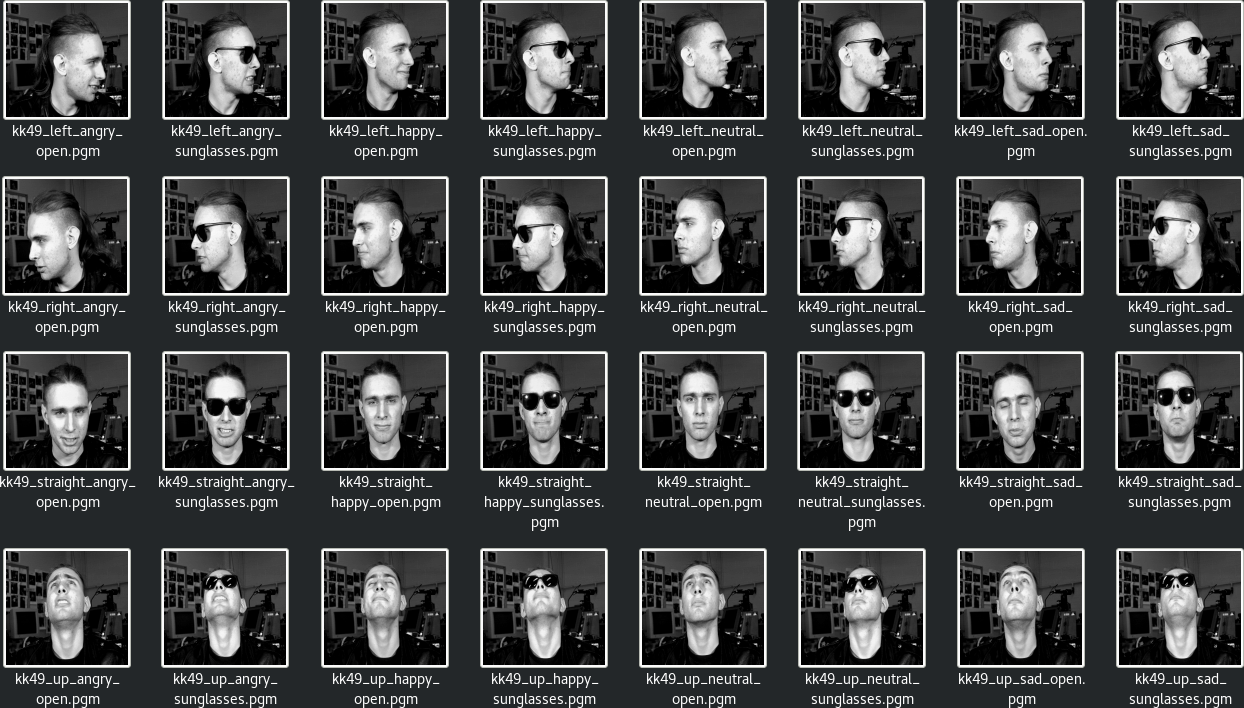
\includegraphics[width=\textwidth]{male}
		\caption[Different poses of a male person]{Different poses of a male person, with and without sunglasses.}
	\end{figure}
	
	\begin{figure}[H]
		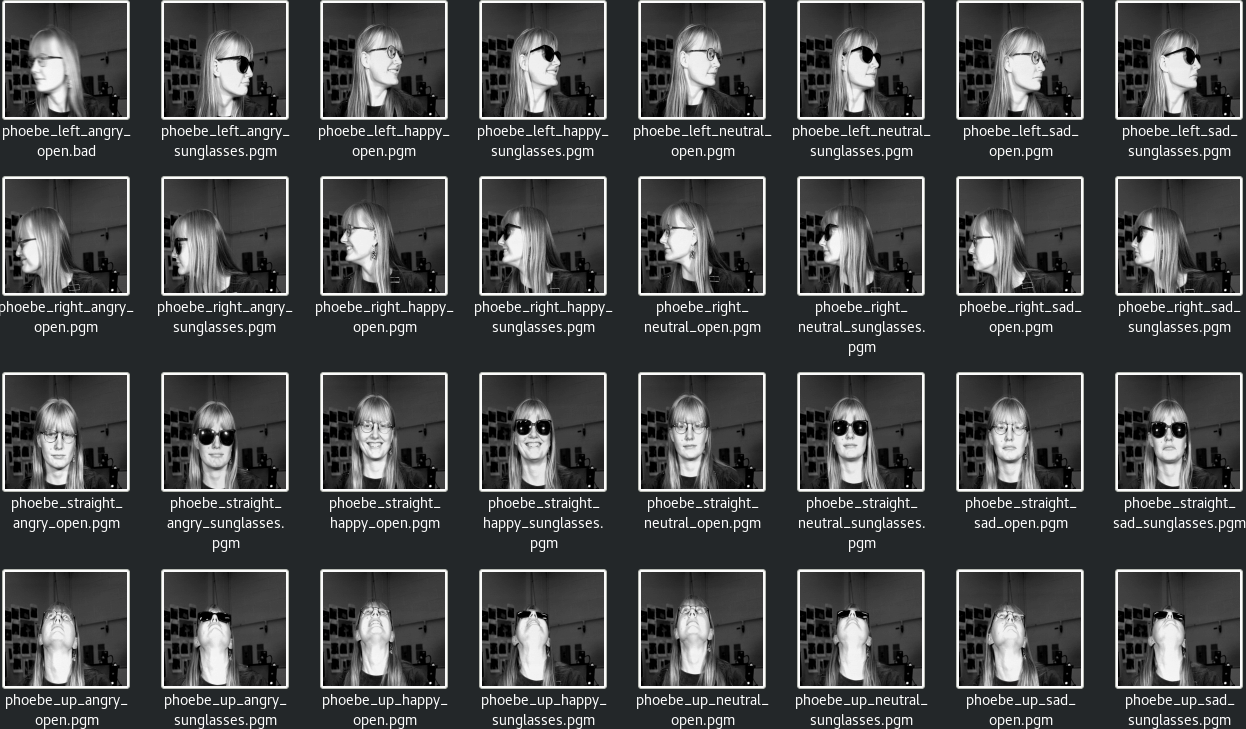
\includegraphics[width=\textwidth]{female}
		\caption[Different poses of a male person]{Different poses of a male person, with and without sunglasses.}
	\end{figure}
	
	The images obey the PGM (portable gray map) format specifications \cite{bib:pgm}.
	
	\begin{figure}[H]
		\centering
		
\includegraphics{sample}
		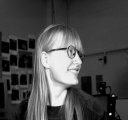
\includegraphics{sample1}
		\caption{Sample PGM images of a smiling male and a smiling female with sunglasses, side view.}
	\end{figure}
	
	When a PGM image is opened in a plain text editor similar text will be as follows:\\
	
	\texttt{P2\\
	24 7\\
	15\\
	0  0  0  0  0  0  0  0  ...\\
	0  3  3  3  3  0  0  7  ...\\
	0  3  0  0  0  0  0  7  ...\\
	0  3  3  3  0  0  0  7  ...\\
	0  3  0  0  0  0  0  7  ...\\
	0  3  0  0  0  0  0  7  ...\\
	0  0  0  0  0  0  0  0  ...\\}
		
	The first three rows of the image are just metadata. Each image are of size 128 * 160 pixels for a total of 15360 attributes and the feature vector is formed row-wise. There are 320 training images (faces without sunglasses) and 320 validation images (faces with sunglasses). After forming the labels and input vectors the ANN and SVM are now ready to train.
	
	\subsection{The Classifiers}
	The code is made using Python, a high level general-purpose programming language that is relatively easy to learn and has very good features in list manipulation. The \texttt{sklearn} library of Python was used. Other libraries used are \texttt{numpy} and \texttt{scipy}.
	
	We have obvious reasons of using existing libraries. More time is dedicated for training the dataset and tuning the parameters instead of implementing the classifier. Source codes released in the open-source community might be better than our own implementation. Continuous contribution of the community through GitHub make \texttt{scikit-learn} library compatitive for machine learning.
	
	In this project \texttt{scikit-learn} will be used for face recognition activity, the most popular machine learning library for Python. \cite{bib:sklearn} It contains simple and efficient tools for data mining and data analysis including classification, regression, clustering, dimensionality reduction, model selection and data preprocessing.
	
	Documentation of \texttt{scikit-learn} for ANN and SVM can be found at \cite{bib:sklearn}. The method signature of \texttt{sklearn.svm.SVC} is as follows:
	
	\texttt{class sklearn.svm.SVC(C=1.0, kernel='rbf', degree=3, gamma='auto', coef0=0.0, \\shrinking=True, probability=False, tol=0.001, cache\_size=200, class\_weight=None,\\ verbose=False, max\_iter=-1, decision\_function\_shape=None, random\_state=None)}
	
	It is a C-Support Vector Classification based on \texttt{libsvm}, where the multiclass support is handled according to a one-vs-one scheme. Linear, polynomial, RBF, sigmoid and precomputed kernels are supported. Relevant attributes and methods used for this research are the following:
	\begin{itemize}
		\item \texttt{fit(X, y)}: fit the SVM model according to the given training data
		\item \texttt{predict(X)}: perform classification on samples in input data X
		\item \texttt{score(X, y)}: returns the mean accuracy on the given test data and labels
		\item \texttt{support\_vectors\_}: returns the list of support vectors of the SVM model
		\item \texttt{n\_support\_}: returns the number of support vectors for each class
	\end{itemize}
	
	The parameter \texttt{gamma} measures how far the influence of a single instance reaches in the multi-dimensional space. Low values mean 'far' and high values meaning 'close'. This can be seen as the inverse of the radius of influence of each instances selected by the model as support vectors \cite{bib:hyp}. The \texttt{C} parameter trades off misclassification against simplicity of the decision surface. A low \texttt{C} makes it smooth while high \texttt{C} aims at classifying training instances correctly by giving the model freedom to select more samples as support vectors \cite{bib:hyp}.
	
	To estimate optimal parameters for the SVM classifier, the \texttt{GridSearchCV} class is used with the following signature:
	
	\texttt{class sklearn.model\_selection.GridSearchCV(estimator, param\_grid, scoring=None, fit\_params=None, n\_jobs=1, iid=True, refit=True, cv=None, verbose=0,\\ pre\_dispatch='2*n\_jobs', error\_score='raise', return\_train\_score=True)}
	
	This class utilizes exhaustive search over specified parameter values for a specific classifier. The parameters of a classifier are optimized by cross-validated grid-search over a parameter grid. Possible parameters are assigned in the \texttt{param\_grid} variable. Initialization of this class is similar below.
	
	\texttt{tuned\_parameters = [{'kernel': ['rbf'], 'gamma': ['auto'] +\\ np.ndarray.tolist(gammas), 'C': C},
		{'kernel': ['linear'], 'C': C},
		{'kernel': ['poly'], 'C': C, 'degree': poly\_d, 'gamma': ['auto'] +\\ np.ndarray.tolist(gammas), 'coef0': coes},
		{'kernel': ['sigmoid'], 'C': C, 'gamma': ['auto'] + np.ndarray.tolist(gammas),\\ 'coef0': coes}]}
	
	\texttt{clf = GridSearchCV(svm(), tuned\_parameters, cv=4, n\_jobs=-1, verbose=10)\\
		clf.fit(X, y)}
	
	Different parameters for SVM are obtained such that it maximizes testing accuracy. Accuracy and running time are performance measures used in comparison. Support vectors will also be extracted from the best SVM model to get the important faces from the dataset.
	
	\section{Results and Discussion}
	
	For a fixed kernel but different parameters, the accuracy of classification changes. The table plot the accuracy of SVM given several hyperparameters. These are some of the results \texttt{GridSearchCV} displayed in optimizing the SVM.
	\begin{center}
	\begin{tabular}{c|c|c}
		\hline
		\head{Kernel} & \head{Param} & \head{Accuracy} (\%)\\
		\hline
		linear & & 88.7500 \\
		polynomial & d=1  & 88.7500 \\
		 & d=2  & 88.7500 \\
		 & d=3  & 89.6875 \\
		 & d=4  & 90.0000 \\
		 & d=5 & 90.6250 \\
		 & d=6  & 89.3750 \\
		 & d=7  & 85.6250 \\
		 & d=8 & 83.1250 \\
		 & d=9  & 80.9375 \\
		 & d=10 & 77.8125 \\
		RBF & g=1/(128*120)  & 29.0625 \\
		sigmoid & g=1/(128*120)  & 5.0000
	\end{tabular}
	\end{center}
	
	Using a polynomial kernel makes the SVM better in generalization. Varying image background (see figures 1 \& 2) is one of the reasons why this classifier did not achieved full accuracy.
	
	It is observed that accuracy is not sensitive to \texttt{gamma}. It is also worth noting that there are 291/320 support vectors from the input data, which means that most of these are support vectors and of similar importance in training the SVM. In fact, each input instance contains unique facial expressions from each person. This is an expected result. Training and testing each SVM instance takes less than a minute.
	
	It is a good idea to treat each pixel as a feature as suggested by literature because each person has different facial features like skin color, shape, etc. Even if one uses sunglasses or change its facial expression, the SVM can nearly recognize the face of that person.
	For the sigmoid function appears to the worst kernel whatever $\gamma$ value is used. The polynomial function is the best SVM kernel for face recognition.
	
	\section{Conclusion}
	It is established that SVM performs better than ANN for the image classification problem involving supervised learning. Another competitor of SVM comes from a class of unsupervised learning methods, the Principal Component Analysis specifically the eigenfaces algorithm \cite{bib:pca}. One can also look for deep learning to solve this problem \cite{bib:img}.
	
	\begin{thebibliography}{9}
		\bibitem{bib:cmu} UCI Machine Learning Repository, \textit{CMU Face Images Data Set}. \url{ https://archive.ics.uci.edu/ml/datasets/CMU+Face+Images}
		
		\bibitem{bib:pgm} J. Poskanzer, \textit{PGM Format Specification.} \url{http://netpbm.sourceforge.net/doc/pgm.html}
		
		\bibitem{bib:fin} K. Kim. \textit{Financial time series forecasting using support vector machines}. Dongguk University, 2003.
		
		\bibitem{bib:cred} Z. Huang, et. al. \textit{Credit rating analysis with support vector machines and neural networks: a market comparative study}. University of Arizona, 2003.
		
		\bibitem{bib:sklearn} scikit-learn, Machine Learning in Python. \url{http://scikit-learn.org/stable/index.html}.
		
		\bibitem{bib:pca} Eigenfaces for Face Recognition \url{http://www.vision.jhu.edu/teaching/vision08/Handouts/case_study_pca1.pdf}
		
		\bibitem{bib:hyp} Plot different SVM classifiers in the iris dataset. \url{http://scikit-learn.org/stable/auto_examples/svm/plot_iris.html#sphx-glr-auto-examples-svm-plot-iris-py}
		
		\bibitem{bib:img} Y. Taigman, M. Yang, M. Ranzato, W. Wolf. \textit{DeepFace: Closing the Gap to Human-Level Performance in Face Verification}. \url{https://research.facebook.com/publications/deepface-closing-the-gap-to-human-level-performance-in-face-verification/}
	\end{thebibliography}
	
\end{document}